\begin{figure}[htpb]
	\centering\capstart{}
	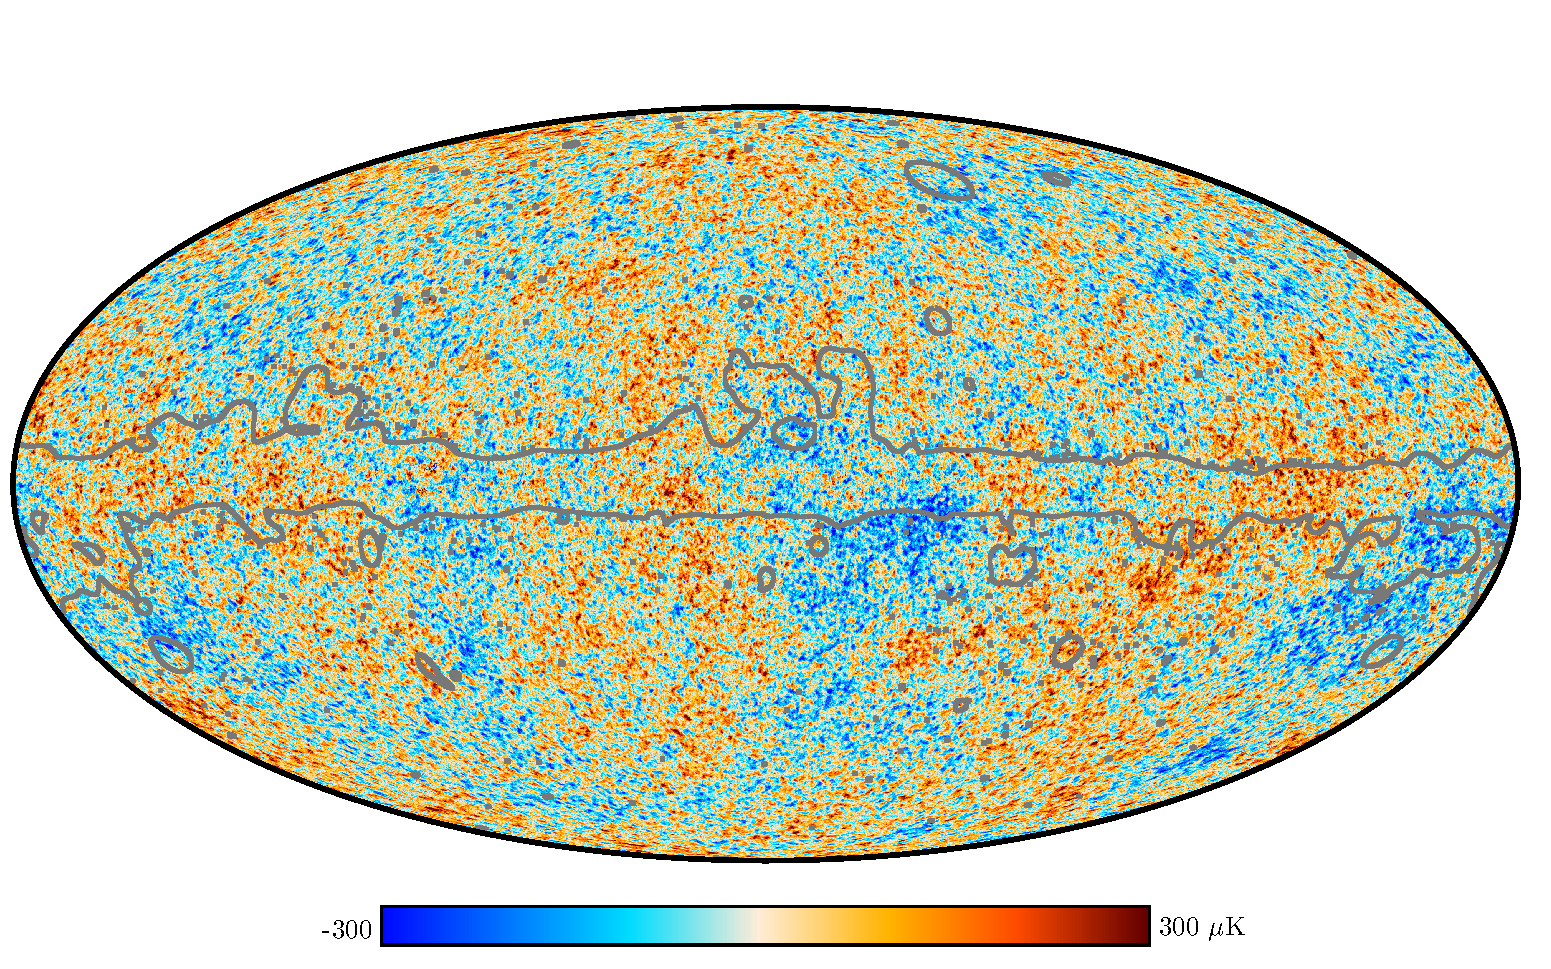
\includegraphics[width=\textwidth]{planck_2018_temp_mask.pdf}
	\caption[
		The 2018 \emph{Planck} CMB map extracted using the \texttt{SMICA} method
	]{
		The \texttt{SMICA}~\cite{Planck2020a} foreground-cleaned temperature map of the \emph{Planck} CMB sky (courtesy of \emph{The Planck Collaboration 2018}~\cite{Planck2020}).
		The CMB map has been masked, primarily around the Galactic plane (outlined in grey), and inpainted in regions where residuals from foreground emission are expected to be considerable.
		Slepian wavelets offer an alternative approach in which the wavelets are constructed in the region outside the mask.
	}\label{fig:chapter2_planck_unmasked}
\end{figure}
